\documentclass[border=2pt]{standalone}
\usepackage{tikz}
\usepackage{amsmath}

\begin{document}
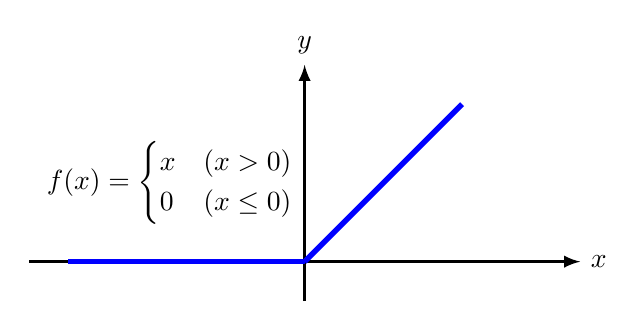
\begin{tikzpicture}[line width=1pt]
    \draw [-latex] (-3.5, 0) -- (3.5, 0) node [right] {$ x $};
    \draw [-latex] (0, -0.5) -- (0, 2.5) node [above] {$ y $};

    \draw [blue, line width=2pt, domain=-3:0, variable=\x] plot({\x}, {0});
    \draw [blue, line width=2pt, domain=0:2, variable=\x] plot({\x}, {\x});

    \node at (-1.7, 1) {
        $ f(x) =
            \begin{cases}
                x & (x > 0)   \\
                0 & (x \le 0)
            \end{cases}
        $
    };
\end{tikzpicture}
\end{document}